\documentclass[a4paper,oneside,11pt]{article}
\usepackage[utf8]{inputenc}  
\usepackage[T1]{fontenc}  
\usepackage[francais]{babel}
\usepackage{textcomp}
\usepackage{amsmath}
\usepackage{amsmath}
\usepackage{listings}
\usepackage[makeroom]{cancel}
\usepackage{lmodern}
\usepackage{algorithm}
\usepackage{algorithmic}
\usepackage{stmaryrd}
\usepackage{upgreek}
\usepackage{dsfont}
\usepackage{graphicx}
\usepackage{caption} 
\usepackage{a4wide}
\usepackage{fullpage} % Package to use full page
\usepackage{parskip} % Package to tweak paragraph skipping
\usepackage{microtype}
\usepackage{tikz} % Package for drawing
\usepackage{hyperref}
\setcounter{tocdepth}{3}
\usepackage{geometry}
\geometry{hmargin=2.5cm,vmargin=1.5cm}
\usepackage{graphicx}
\usepackage{epsf}
\usepackage{epsfig}
\usepackage{amssymb, amsmath, amsopn, amstext, amscd, amsthm, amsfonts}
\usepackage{version}
\usepackage{todonotes}
\usepackage{xcolor}
%\usepackage{minted}
\usepackage{shortvrb,moreverb,tcolorbox}
\usepackage{ mathrsfs }
\usepackage{listings}
\usepackage{multicol}
\usepackage{sectsty}
\usepackage{dsfont}

\makeatletter
\newsavebox\tboxa
\newsavebox\tboxb
\newlength\tdima

\newcommand{\ds}{\ensuremath{\displaystyle}}
\newcommand{\R}{\ensuremath{\mathbb{R}}}
\newcommand{\E}{\ensuremath{\mathbb{E}}}
\newcommand{\Om}{\ensuremath{\mathcal{O}}}
\newcommand{\Var}{\ensuremath{\operatorname{Var}}}
\newcommand{\var}{\ensuremath{\operatorname{var}}}
\newcommand{\Arg}{\ensuremath{\operatorname{Arg}}}
\newcommand{\dr}{\ensuremath{\partial}}
\newcommand{\C}{\ensuremath{\mathbb{C}}}
\newcommand*{\ov}{\mathpalette\@ov}
\newcommand{\Tr}{\ensuremath{\operatorname{Trace}}}
%partie réelle d'un complexe
\renewcommand{\Re}{\operatorname{Re}}

%partie imaginaire d'un complexe
\renewcommand{\Im}{\operatorname{Im}}

\newcommand{\dsum}[2]{\sum\limits_{#1}^{#2}}

\newcommand*{\@ov}[2]{%
    \sbox{\tboxa}{$\m@th#1\mathrm{#2}$}%
    \setbox\tboxb\null%
    \ht\tboxb\ht\tboxa%
    \dp\tboxb\dp\tboxa%
    \wd\tboxb\wd\tboxa%
    \sbox{\tboxa}{$\m@th#1{#2}$}%
    \setlength\tdima{\the\wd\tboxa}%
    \addtolength\tdima{-\the\wd\tboxb}%
    \sbox{\tboxb}{$\m@th#1\hskip\tdima\overline{\xusebox{\tboxb}}$}
    \rlap{\usebox\tboxb}{\usebox\tboxa}}

\lstset{upquote=true,columns=flexible,basicstyle=\ttfamily}

\lstset{language={[LaTeX]TeX},texcsstyle=*\color{blue},commentstyle=\color{gray}}

\lstset{language={Python},texcsstyle=*\color{blue},commentstyle=\color{gray},frame =tBlR ,rulesep =1mm ,framesep =5mm,framerule =2pt,
xrightmargin =4mm,xleftmargin =4mm ,rulecolor ={\color [gray]{0.6}},rulesepcolor={\color [gray]{0.9}},numberstyle=\tiny\color{red},backgroundcolor=\color{lightcyan}}

\lstnewenvironment{code-Python}[1][]{
	\lstset{
	language={Python},
	upquote=true,
	columns=flexible,
	showstringspaces=false,% do not replace spaces in strings by a certain character 
    captionpos=b,% positioning of the caption below 
    breaklines=true,% automatic line breaking 
	basicstyle=\ttfamily,
	texcsstyle=*\color{blue},
	commentstyle=\color{gray},
	keywordstyle=\color{blue},
	stringstyle=\color{red},
	numberstyle=\tiny\color{red},
	moretexcs={abslabeldelim,setlength,abstitleskip}
	alsoletter={.<-},% becomes a letter 
    alsoother={$},% becomes other 
    otherkeywords={!=, ~, $,\&, \%/\%, \%*\%, \%\%, <-, <<-, /},% other keywords 
    deletekeywords={c}% remove keywords
	#1
	}
} {}


\newcommand*{\xusebox}[1]{\mathord{{\usebox{#1}}}}

\newcommand*{\colorboxed}{}
\def\colorboxed#1#{%
  \colorboxedAux{#1}%
}
\newcommand*{\colorboxedAux}[3]{%
  % #1: optional argument for color model
  % #2: color specification
  % #3: formula
  \begingroup
    \colorlet{cb@saved}{.}%
    \color#1{#2}%
    \boxed{%
      \color{cb@saved}%
      #3%
    }%
  \endgroup
}

\definecolor{lavendermist}{rgb}{0.9, 0.9, 0.98}
\definecolor{lightcyan}{rgb}{0.91, 1.0, 1.0}
\definecolor{gainsboro}{rgb}{0.86, 0.86, 0.86}


\DeclareMathOperator{\ind}{\perp \!\!\! \perp}

\title{Rapport de méthodes numériques pour l'actuariat}


\author{Chevaux Alexandre // Garrigue Matthieu}
\date{}

\DeclareMathOperator{\e}{e}

\subsectionfont{\large\bfseries\underline}
\begin{document}

\maketitle


\part*{Projet 4: Incertitude en polynôme du chaos}
\addcontentsline{toc}{part}{\protect\numberline{}Projet 4: Incertitude en polynôme du chaos}%

\qquad On cherche à mesurer l'impact de l'incertitude $\sigma$ sur le calcul du Best Estimate et sur le coût de la garantie associée.

On rappelle que la valeur économique notée $\phi$ est la solution de:
\begin{equation}
\label{EDPphi}
\frac{\dr \phi}{\dr t}+\frac{\sigma^2}{2}\frac{\dr^2 \phi}{\dr x^2}+k(x_{\infty}-x)\frac{\dr \phi}{\dr x}+x\phi +(1-g)\phi=0
\end{equation} 

Dans notre cas $\phi$ est dépendante du paramètre incertain $\sigma$.
On modélise $\sigma$ par un bruit gaussien:
\begin{equation}
\sigma^2=\sigma^{2}(\xi)=(\mu +\nu\xi)^{2}, \xi \backsim \mathcal{N}(0,1)
\end{equation}

\underline{(i) Déterminer le système linéaire bloc (d+1)$\times$(d+1) couplant les EDP:}

On prendra dans notre cas \textbf{d=2} autrement dit, on se restreindra aux termes $\phi_k$ avec $k \leq 2$ pour des raisons numériques.

On a 
\begin{equation}
\label{exprphi}
\phi(x,t,\xi)=\sum_{j\ge 0}\phi_{j}(x,t)H_{j}(\xi)
\end{equation}
avec $(H_{n})_{n\ge0}$ la famille des polynômes de Hermite

On multiplie (\ref{EDPphi}) par $H_k$ et on appliquera ensuite l'espérance à chaque terme. Cela nous permettra d'obtenir un système linéaire.
\begin{equation}
\phi(x,t,\xi)=\sum_{j\ge 0}\phi_{j}(x,t)H_{j}(\xi)
\end{equation}
On rappelle que: 
\begin{equation}
\label{espHmHn}
\E(H_m(\xi)H_n(\xi)) = \delta_{m,n}n!
\end{equation}

On utilisera tout au long de ces calculs les résultats d'espérance de puissances de $\xi$. \newline
En effet, on peut noter que $\E[\xi^{n+1}]=0\ \forall n \in \mathds{N}$
Pour les puissances paires, les résultats sont moins immédiats:
\begin{align*}
\E(\xi^2) &= \E(\xi)^2+\Var(\xi)=1 \\
\E(\xi^4) &= 3 \text{ par intégration par parties}\\
\E(\xi^6) &= 15 \text{ en utilisant la formule générale de l'espérance des puissance paires} \\ &\text{d'une variable aleatoire normale centrée réduite.}
\end{align*}
Par ailleurs, on utilisera aussi les propriétés sur les polynômes de l'Hermite, autrement dit $H_{n+1}=X H_n-nH_{n-1}\quad H_0=1,\; H_1=X \; n \geq 1$ \newline 
On utilisera également la linéarité de l'espérance ainsi que les propriétés  (\ref{espHmHn})et (\ref{exprphi})

\underline{Pour $H_{0}$:} \newline
On va appliquer
\begin{align*}
&\mathbb{E}\left[\frac{\dr \phi}{\dr t}+\frac{\sigma^2}{2}\frac{\dr^2 \phi}{\dr x^2}+k(x_{\infty}-x)\frac{\dr \phi}{\dr x}+x\phi +(1-g)\phi\right]=0 \\
&\Leftrightarrow \frac{\dr \phi_{0}}{\dr t}\times1+\frac{\dr \phi_{1}}{\dr t}\times0\frac{\dr \phi_{2}}{\dr t}\times 0 +\mathbb{E}\left[\frac{(\mu+\nu\xi)^{2}}{2}\left(\frac{\dr^{2}\phi_{0}}{\dr x^{2}} \times 1+\frac{\dr^{2}\phi_{1}}{\dr x^{2}} \times \xi+\frac{\dr^{2}\phi_{2}}{\dr x^{2}} \times (\xi^{2}-1)\right)\right] \\    &+k(x_{\infty}-x)\frac{\dr \phi_{0}}{\dr x} \times1 +x(\phi_{0})+(1-g)\phi_{0}=0
\end{align*}
Distribuons avec le terme $\ds{\frac{(\mu+\nu\xi)^{2}}{2}}$ et appliquons la linéarité de l'espérance. \newline 
On utilisera par ailleurs les résultats sur l'espérance des puissances de $\xi$ donnés plus haut. \newline

Ainsi, on obtient finalement, \newline
\underline{EDP en $H_{0}$:}

$\colorboxed{red}{\ds{\frac{\dr \phi_{0}}{\dr t} +\frac{\dr^{2}\phi_{0}}{\dr x^{2}}(\frac{\mu^{2}+\nu^{2}}{2})+\frac{\dr^{2}\phi_{1}}{\dr x^{2}}(\mu\nu)+\frac{\dr^{2}\phi_{2}}{\dr x^{2}}\times \nu^2+k(x_{\infty}-x)\frac{\dr \phi_{0}}{\dr x} +x\phi_{0}+(1-g)\phi_{0}=0}}$

\underline{Pour $H_{1}$:}

$\ds{\mathbb{E}\left[\frac{\dr \phi }{\dr t}H_{1}\right]=\mathbb{E}\left[\frac{\dr\phi_{0}}{\dr t}H_{0}H_{1}\right]+\mathbb{E}\left[\frac{\dr\phi_{1}}{\dr t}H_{1}^{2}\right]\mathbb{E}\left[\frac{\dr\phi_{2}}{\dr t}H_{2}H_{1}\right]}$

\underline{1er terme:}
\begin{equation*}
\cancel{\frac{\dr \phi_{0}}{\dr t}\times0}+\frac{\dr \phi_{1}}{\dr t}\times1+\cancel{\frac{\dr \phi_{2}}{\dr t}\times0}
\end{equation*}

On utilisera pour le calcul du deuxième terme les résultats sur l'espérance des puissance de $\xi$, la linéarité de l'espérance et le résultat donnés en (\ref{espHmHn})\newline
\underline{2ème terme:}
\begin{align*}
&\mathbb{E}\left[\frac{\sigma^{2}}{2}(\frac{\dr^{2}\phi_{0}}{\dr x^{2}}H_{0}H_{1})\right]+\mathbb{E}\left[\frac{\sigma^{2}}{2}\frac{\dr^{2}\phi_{1}}{\dr x^{2}}H_{1}^2\right]+\mathbb{E}\left[\frac{\sigma^{2}}{2}\frac{\dr^{2}\phi_{1}}{\dr x^{2}}H_{2}H_{1}\right] \\
&=\mathbb{E}\left[\frac{\mu+2\mu\nu\xi+\mu^{2}\xi^{2}}{2}\frac{\dr^{2}\phi_{0}}{\dr x^{2}}H_{0}H_{1}\right] \\
&+\mathbb{E}\left[\frac{\mu+2\mu\nu\xi+\mu^{2}\xi^{2}}{2}\frac{\dr^{2}\phi_{1}}{\dr x^{2}}H_{1}^{2}\right] \\
&+\mathbb{E}\left[\frac{\mu+2\mu\nu\xi+\mu^{2}\xi^{2}}{2}\frac{\dr^{2}\phi_{1}}{\dr x^{2}}H_{2}H_{1}\right] \\
&=\frac{\dr^{2}\phi_{0}}{\dr x^{2}}\mathbb{E}\left[\frac{\mu^{2}\xi+2\mu\nu\xi^{2}+\mu^{2}\xi^{2}}{2}\right] \\
&+\frac{\dr^{2}\phi_{1}}{\dr x^{2}}\mathbb{E}\left[\frac{\mu^{2}\xi^{2}+2\mu\nu\xi^{3}+\mu^{2}\xi^{4}}{2}\right] \\
&+\frac{\dr^{2}\phi_{2}}{\dr x^{2}}\mathbb{E}\left[\frac{\mu^{2}(\xi^{3}-\xi)+2\mu\nu(\xi^{4}-\xi^{2})+\mu^{2}(\xi^{5}-\xi^{3})}{2}\right] \\
&=\frac{\dr^{2}\phi_{0}}{\dr x^{2}}\mu\nu+\frac{\dr^{2}\phi_{1}}{\dr x^{2}}\frac{\mu^{2}+3\nu^{2}}{2}+\frac{\dr^{2}\phi_{2}}{\dr x^{2}}\times 2 \mu \nu
\end{align*}

\underline{3ème terme:}
$\ds{k(x_{\infty}-x)\frac{\dr \phi_{1}}{\dr x}}\newline$

\underline{4ème terme:}
\begin{align*}
&\mathbb{E}\left[x\phi H_{1}\right]=x \mathbb{E}\left[\phi_{0}H_{0}H_{1}\right]+x \mathbb{E}\left[\phi_{1}H_{1}^{2}\right]+x \mathbb{E}\left[\phi_{2}H_{2}H_{1}\right] \\
&=x\phi_{1}
\end{align*}

\underline{5ème terme:}
\begin{align*}
\mathbb{E}\left[(1-g)\phi H_{1}\right]=(1-g)\phi_{1}
\end{align*}

\underline{EDP en $H_{1}$:}

$\colorboxed{red}{\ds{\frac{\dr \phi_{1}}{\dr t} +\frac{\dr^{2}\phi_{0}}{\dr x^{2}}\mu\nu+\frac{\dr^{2}\phi_{1}}{\dr x^{2}}(\frac{\mu^{2}+3\nu^{2}}{2})+\frac{\dr^{2}\phi_{2}}{\dr x^{2}}\times 2 \mu \nu+k(x_{\infty}-x)\frac{\dr \phi_{1}}{\dr x} +x\phi_{1}+(1-g)\phi_{1}=0}}$

\underline{Pour $H_{2}$:} \newline
\underline{1er terme:}
\begin{align*}
&\mathbb{E}\left[\frac{\dr \phi}{\dr t}H_{2}\right]=\cancel{\frac{\dr \phi_{0}}{\dr t}\mathbb{E}\left[H_{0}H_{2}\right]}+\cancel{\frac{\dr \phi_{1}}{\dr t}\mathbb{E}\left[H_{1}H_{2}\right]}+\frac{\dr \phi_{2}}{\dr t}\mathbb{E}\left[H_{2}^{2}\right] \\
&=\frac{\dr \phi_{2}}{\dr t}\times2!=\frac{\dr \phi_{2}}{\dr t}\times2
\end{align*}

\underline{2ème terme:}
\begin{align*}
&\mathbb{E}\left[\frac{\sigma^{2}}{2}(\frac{\dr^{2}\phi}{\dr x^{2}}H_{2})\right] \\
&=\mathbb{E}\left[\frac{(\mu^{2}+2\mu\nu\xi+\mu^{2}\xi^{2})}{2}\right]\left(\frac{\dr^{2}\phi_{0}}{\dr x^{2}}H_{0}H_{2}+\frac{\dr^{2}\phi_{1}}{\dr x^{2}}H_{1}H_{2}+\frac{\dr^{2}\phi_{0}}{\dr x^{2}}H_{2}^{2}\right) \\
&=\cancel{\frac{\dr^{2}\phi_{0}}{\dr x^{2}}(0)}+\frac{\dr^{2}\phi_{1}}{\dr x^{2}}(2 \mu \nu)+\frac{\dr^{2}\phi_{2}}{\dr x^{2}} \times \left[\frac{(\mu^{2}+2\mu\nu\xi+\mu^{2}\xi^{2})}{2}\right] \times (\xi^4-2 \xi^2+1) \\
&=\frac{\dr^{2}\phi_{1}}{\dr x^{2}}(2 \mu \nu)+\frac{\dr^{2}\phi_{2}}{\dr x^{2}} \left( \mu^2 + \E \left( \frac{(\xi^6-2\xi^4+\xi^2)\nu^2}{2} \right) \right) \\
&=\frac{\dr^{2}\phi_{1}}{\dr x^{2}}(2 \mu \nu)+\frac{\dr^{2}\phi_{2}}{\dr x^{2}} \left( \mu^2 + \E \left( \frac{15-6+1}{2} \nu^2 \right) \right) \\
&=\frac{\dr^{2}\phi_{1}}{\dr x^{2}}\times(2 \mu \nu)+\frac{\dr^{2}\phi_{2}}{\dr x^{2}} \times ( \mu^2 + 5 \nu^2)  
\end{align*}

\underline{3ème terme:}
\begin{align*}
\mathbb{E}\left[k(x_{\infty}-x)\frac{\dr \phi}{\dr x}H_{2}\right]=k(x_{\infty}-x)2\frac{\dr \phi_{2}}{\dr t}
\end{align*}
\underline{4ème terme:} 
\begin{align*}
\mathbb{E}\left[x\phi H_{2}\right]=x\phi_{2}\times2
\end{align*}
\underline{5ème terme:} 
\begin{align*}
\mathbb{E}\left[(1-g)\phi H_{2}\right]=2(1-g)\phi_{2}
\end{align*}


\underline{EDP en $H_{2}$:}

$\colorboxed{red}{ \ds{2\frac{\dr \phi_{2}}{\dr t} +\frac{\dr^{2}\phi_{1}}{\dr x^{2}}\times(2 \mu \nu)+\frac{\dr^{2}\phi_{2}}{\dr x^{2}} \times ( \mu^2 + 5 \nu^2)  +2k(x_{\infty}-x)\frac{\dr \phi_{2}}{\dr x} +2x\phi_{2}+2(1-g)\phi_{2}=0}}$



Finalement, on a le système linéaire suivant:\newline

$\left\{
    \begin{array}{ll}
        \cdot\ \ds{\frac{\dr \phi_{0}}{\dr t} +\frac{\dr^{2}\phi_{0}}{\dr x^{2}}(\frac{\mu^{2}+\nu^{2}}{2})+\frac{\dr^{2}\phi_{1}}{\dr x^{2}}(\mu\nu)+\frac{\dr^{2}\phi_{2}}{\dr x^{2}}\times \nu^2+k(x_{\infty}-x)\frac{\dr \phi_{0}}{\dr x} +x\phi_{0}+(1-g)\phi_{0}=0} \\\\
        \cdot\ \ds{\frac{\dr \phi_{1}}{\dr t} +\frac{\dr^{2}\phi_{0}}{\dr x^{2}}\mu\nu+\frac{\dr^{2}\phi_{1}}{\dr x^{2}}(\frac{\mu^{2}+3\nu^{2}}{2})+\frac{\dr^{2}\phi_{2}}{\dr x^{2}}\times 2 \mu \nu+k(x_{\infty}-x)\frac{\dr \phi_{1}}{\dr x} +x\phi_{1}+(1-g)\phi_{1}=0} \\\\
        \cdot\ \ds{2\frac{\dr \phi_{2}}{\dr t} +\frac{\dr^{2}\phi_{1}}{\dr x^{2}}\times(2 \mu \nu)+\frac{\dr^{2}\phi_{2}}{\dr x^{2}} \times ( \mu^2 + 5 \nu^2)  +2k(x_{\infty}-x)\frac{\dr \phi_{2}}{\dr x} +2x\phi_{2}+2(1-g)\phi_{2}=0} 
    \end{array}
\right.$
\newline \newline \newline \newline
Ecrivons le sous forme matricielle:
$$
\hspace*{-0.1\textwidth}
\begin{pmatrix}
\scriptstyle \dr_t \phi_0 \\
\scriptstyle \dr_t \phi_1 \\
\scriptstyle 2 \dr_t \phi_2
\end{pmatrix}  
+
\begin{pmatrix} 
\scriptstyle x +(1-g) & \scriptstyle k(x_{\infty}-x) &  \frac{\mu^{2}+\nu^{2}}{2} & \scriptstyle 0 & \scriptstyle 0 & \scriptstyle \mu \nu & \scriptstyle 0 & \scriptstyle 0 & \scriptstyle \nu^2\\
\scriptstyle 0 & \scriptstyle 0 & \scriptstyle \mu \nu & \scriptstyle x + (1-g) & \scriptstyle k(x_{\infty}-x) &  \frac{\mu^{2}+3\nu^{2}}{2} & \scriptstyle 0 & \scriptstyle 0 & \scriptstyle 2\mu \nu \\
\scriptstyle 0 & \scriptstyle 0 & \scriptstyle 0 & \scriptstyle 0 & \scriptstyle 0 & \scriptstyle 2 \mu \nu & \scriptstyle 2(x+(1-g)) & \scriptstyle 2k(x_{\infty}-x) & \scriptstyle \mu^2 + 5 \nu^2 
\end{pmatrix}
\times 
\begin{pmatrix}
\scriptstyle \phi_0 \\
\scriptstyle \dr_x \phi_0 \\
\scriptstyle \dr_x^2 \phi_0 \\
\scriptstyle \phi_1 \\
\scriptstyle \dr_x \phi_1 \\
\scriptstyle \dr_x^2 \phi_1 \\
\scriptstyle \phi_2 \\
\scriptstyle \dr_x \phi_2 \\
\scriptstyle \dr_x^2 \phi_2 
\end{pmatrix}
= \begin{pmatrix}
\scriptstyle 0 \\ \scriptstyle 0 \\ \scriptstyle 0
\end{pmatrix}
$$

De manière générale, le problème peut se ramener à \textbf{une structure penta-diagonale bloc} avec une implémentation qui se fait en deux parties, représentant l'EDP pour la partie intérieure et prenant en comtpe les conditions au bord pour la partie exterieure. \newline
Pour la partie exterieure, en se basant sur les conditions aux bords (Neumann, Dirichlet et imposer que $\frac{\partial \phi}{\partial x^2}=0$), il nous sera possible d'obtenir les équations manquantes pour fermer le système.


\underline{(ii) Déterminer le $Best$ $Estimate$ moyen à t=0:}

On rappelle que le $Best$ $Estimate$ est $\mathbb{E}[\phi(x,0,\xi)]$

Comme $\ds{\phi_{k}(x,t)=\mathbb{E}(\phi,x,t,\xi)\frac{H_{k}(\xi)}{k!}}$

$\ds{\mathbb{E}[\phi(x,0,\xi)]=\mathbb{E}(\phi,x,0,\xi)\frac{H_{0}(\xi)}{0!}=\phi_{0}(x,0)}$

Or $\phi_{0}(x,0)$ vérifie:

$\ds{\frac{\dr \phi_{0}}{\dr t} +\frac{\dr^{2}\phi_{0}}{\dr x^{2}}(\frac{\mu^{2}+\nu^{2}}{2})+\frac{\dr^{2}\phi_{1}}{\dr x^{2}}(\mu\nu)+k(x_{\infty}-x)\frac{\dr \phi_{0}}{\dr x} +x\phi_{0}+(1-g)\phi_{0}=0}$

On résout donc cette équation à t=0.

Pour cela, nous allons utiliser une méthode des différences finies:

Nous allons discrétiser l'intervalle [0,L] en n points de pas $h=\frac{L}{n}$ et on fait de même pour l'intervalle de temps $h^{'}=\frac{T}{n}$
On discrétise les dérivées partielles:

$\ds{\frac{\dr \phi_{0}}{\dr t}(x_{i},t_{j})=\frac{\phi{0}(x_{i},t_{j+1})-\phi{0}(x_{i},t_{j})}{h^{'}}}$

$\ds{\frac{\dr^{2} \phi_{0}}{\dr x^{2}}(x_{i},t_{j})=\frac{\phi{0}(x_{i-1},t_{j})+\phi{0}(x_{i+1},t_{j})-2\phi{0}(x_{i},t_{j})}{h^{2}}}$

On peut ainsi avoir une formule de $\phi{0}(x_{i},t_{j+1})$ en fonction de $\phi_{0}(x_{i-1},t_{j})$ et $\phi_{0}(x_{i+1},t_{j})$

Par soucis de simplification, on va considérer trois hypothèses:

$\ds{\frac{\partial^{2}\phi_{1}}{\partial x^{2}}=0}$

$\ds{\frac{\partial^{2}\phi_{1}}{\partial x^{2}}=0}$

$u(0)=0$

L'équation est donc:

$\ds{\frac{\partial\phi_{0}}{\partial t} +\frac{\partial^{2}\phi_{0}}{\partial x^{2}}(\frac{\mu^{2}+\nu^{2}}{2})++k(x_{\infty}-x)\frac{\partial \phi_{0}}{\partial x} +x\phi_{0}+(1-\eta x)\phi_{0}=0}$

$\Leftrightarrow \ds{\frac{\partial\phi_{0}}{\partial t} +\frac{\partial^{2}\phi_{0}}{\partial x^{2}}(\frac{\mu^{2}+\nu^{2}}{2})+kx_{\infty}\frac{\partial \phi_{0}}{\partial x}-x\frac{\partial \phi_{0}}{\partial x} +(1-\eta)x\phi_{0}+\phi_{0}=0}$

On va écrire notre équation sous la forme d'un produit matriciel tel que:

$$\begin{pmatrix} 
\phi_{0}(1,j+1) \\
\phi_{0}(2,j+1) \\
\phi_{0}(3,j+1) \\
... \\
\phi_{0}(n-1,j+1) \\
\phi_{0}(n,j+1)
\end{pmatrix}
=\left((\frac{\mu^{2}+\nu^{2}}{2})
\begin{pmatrix} 
-2 & 1 & 0 & ... & ... & 0 \\
1 & -2 & 1  & 0 & ... & 0\\
0 & ... & ... & ... & ... & 0\\
... & ... & ... & ... & ... & 0 \\
 0 & ... & 0 & 1 & -2 & 1 \\
 0 & ... & ... & 0 & 1 & -2 
\end{pmatrix}
+(kx_{\infty})
\begin{pmatrix} 
-1 & 0 & ... & ... & ... & 0 \\
1 & -1 & 0  & ... & ... & 0\\
0 & ... & ... & ... & ... & 0\\
... & ... & ... & ... & ... & 0 \\
 0 & ... & 0 & 1 & -1 & 0 \\
 0 & ... & ... & ... & 0 & -1 
\end{pmatrix}
\right)
$$
$$
\hspace*{-0.05\textwidth}
+\left(\begin{pmatrix} 
0 & ... & ...  & ... & 0 \\
k & -k & 0   & ... & 0\\
0 & 2k & -2k  & ... & 0\\
... & ... & ...  & ... & 0 \\
 ... &  0 & (n-1)k & -(n-1)k & 0 \\
 0 & ...  & ... & 0 & -nk 
\end{pmatrix}
+\begin{pmatrix} 
0 & ... & ... & ...  & 0 \\
0 & -(1-\eta) & 0  & ... & 0\\
0 & 0 & -2(1-\eta) & ... & 0\\
... & ... & ...  & ... & 0 \\
 0 & ...  & 0 & -(n-1)(1-\eta) & 0 \\
 0 & ... & ... & 0 & -n(1-\eta)
\end{pmatrix}
+Id\right)
$$
$$
\times
\begin{pmatrix} 
\phi_{0}(1,j) \\
\phi_{0}(2,j) \\
\phi_{0}(3,j) \\
... \\
\phi_{0}(n-1,j-1) \\
\phi_{0}(n,j)
\end{pmatrix}
$$

Nous pouvons maintenant mettre en place le code:



\underline{Matrice tridiagonale:}
\begin{code-Python}
### Construction de la matrice tridiagonale
T=1
S_0=1
x_max=2*S_0
m=10
dt=T/n
dx=x_max/m
##2eme terme
mat_tridiag=np.eye(m)*2+np.eye(m,k=1)+ np.eye(m,k=-1)
mat_tridiag=mat_tridiag*((mu*mu+nu*nu)/2)
##3eme terme
iden_2=-np.eye(m)+np.eye(m,k=-1)
iden_2=iden_2*(k*x_inf)
###4eme terme
iden= np.eye(m)+np.eye(m,k=-1)
cpt_row=0
cpt_col=0
for i in iden:
    iden[cpt_row,cpt_col-1]=k*cpt_row
    iden[cpt_row,cpt_col]=-k*cpt_row
    cpt_row=cpt_row+1
    cpt_col=cpt_col+1
##5eme terme
iden_3=np.eye(m)
cpt_row=0
cpt_col=0
for i in iden_3:
    iden[cpt_row,cpt_col]=(1-eta)*cpt_row
    cpt_row=cpt_row+1
    cpt_col=cpt_col+1
##6eme terme
iden_3=np.eye(m)
\end{code-Python}

\underline{Conditions initiales:}
\begin{code-Python}
iden[len(iden)-1]=0
iden_2[len(iden_2)-1]=0
iden_3[len(iden_3)-1]=0
mat_tridiag[len(mat_tridiag)-1]=0
\end{code-Python}

\underline{Matrice obtenue:}

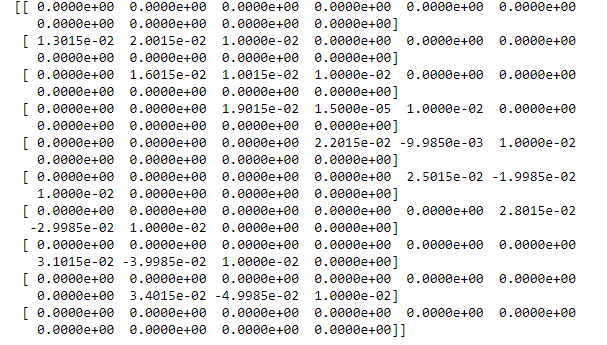
\includegraphics[width=0.5\textwidth]{Image/matrice}

\underline{Code des simulations:}
\begin{code-Python}
U=[]
U=[np.sin(np.pi*k/x_max) for k in np.linspace(0,x_max,m)]
V=np.dot(mat,U)
plt.plot(V)
\end{code-Python}

\underline{Résultat de la simulation:}

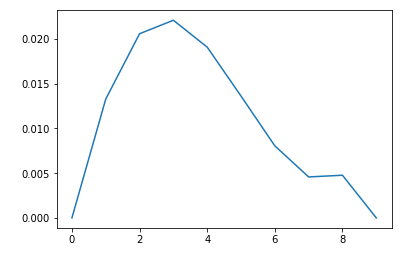
\includegraphics[width=0.5\textwidth]{Image/Simulation}
\end{document}

